\documentclass{beamer}
\usepackage{graphicx}
\usepackage{amsmath}
\usepackage{amsfonts}
\usepackage{amssymb}
\usepackage{tikz}
\usepackage{animate}
\usepackage{media9}
\usetheme{Madrid}
\usepackage{graphicx}   % For minipage alignment
\usepackage{multirow}   % For multi-row cells in tables
\usepackage{amssymb}    % For symbols like \cmark and \xmark
\usepackage{booktabs}   % (Optional) For better table aesthetics
\usepackage{natbib}
\usepackage{tikz}

\usetheme{Madrid}

% 2) Define your custom base color by RGB
\usepackage{xcolor}  % needed if you define custom colors
\definecolor{myprimary}{RGB}{4,130,153} % Example: SteelBlue
\newcommand{\redify}[1]{\textcolor{myprimary}{\textbf{#1}}}
\newcommand{\posterior}{p (\theta \vert \mathcal{D})}
\newcommand{\prior}{p (\theta)}
\newcommand{\likelihood}{p(\mathcal{D} \vert \theta)}
\newcommand{\data}{\mathcal D}
\newcommand{\thetamap}{\theta_{\text{MAP}}}
\newcommand{\hessian}{\nabla_\theta^2 \mathcal{L}(\theta; \mathcal{D})}

\newcommand{\cmark}{\ding{51}}
\newcommand{\xmark}{\ding{55}}


% \newcommand*\circled[1]{\tikz[baseline=(char.base)]{
%             \node[shape=circle,draw,inner sep=2pt] (char) {#1};}}
\newcommand{\circled}[1]{%
  \tikz[baseline=(char.base)]\node[draw,circle,inner sep=1pt,thick](char){\textbf{#1}};%
}

% 3) Override key color settings in Beamer
\setbeamercolor{structure}{fg=myprimary}% affects titles, bullets, etc.
\setbeamercolor{title}{fg=white,bg=myprimary}
\setbeamercolor{subtitle}{fg=myprimary}
\setbeamercolor{frametitle}{fg=white,bg=myprimary!85}
\setbeamercolor{block title}{fg=white,bg=myprimary!75}
\setbeamercolor{block body}{bg=myprimary!10, fg=black}
\setbeamercolor{itemize item}{fg=myprimary}
\setbeamercolor{itemize subitem}{fg=myprimary}
\setbeamercolor{alerted text}{fg=red!80!black} 

\title{Shaping Laser Pulses with Reinforcement Learning}
\author{Francesco Capuano, Davorin Peceli, Gabriele Tiboni}
\date{\today}

\titlegraphic{
  % \includegraphics[width=3cm]{images/RL_logo.png}
}

\begin{document}

%----------------------------------
\begin{frame}
  \titlepage
\end{frame}

%---------------------------------------
\begin{frame}{Overview}
\begin{columns}[T,totalwidth=\textwidth]
    \begin{column}{0.5\textwidth}
        \begin{itemize}
            \item \textbf{The problem}: Shaping laser pulses for high-intensity physics is complex.
            \item Traditional methods are slow and not robust to changes.
            \item \textbf{Our solution}: Use Reinforcement Learning to control the laser.
            \item Our method learns from images, adapts to changes, and is safe.
        \end{itemize}
    \end{column}
    \begin{column}{0.5\textwidth}
        % \begin{figure}
        %     \includegraphics[width=\linewidth]{images/Figure1_and_CPA.png}
        %     \caption{The RL setup for laser pulse shaping.}
        % \end{figure}
    \end{column}
\end{columns}
\end{frame}

%---------------------------------------
\begin{frame}{Background: Shaping Laser Pulses}
\begin{columns}[T,totalwidth=\textwidth]
    \begin{column}{0.5\textwidth}
        \begin{itemize}
            \item Attosecond laser pulses are the shortest events created by mankind.
            \item They provide unprecedented insights into light-matter interactions.
            \item Phase shifts are applied for higher intensities, exploiting non-linear effects.
            \item This is done using a technique called Chirped Pulse Amplification (CPA).
        \end{itemize}
    \end{column}
    \begin{column}{0.5\textwidth}
        % \begin{figure}
        %     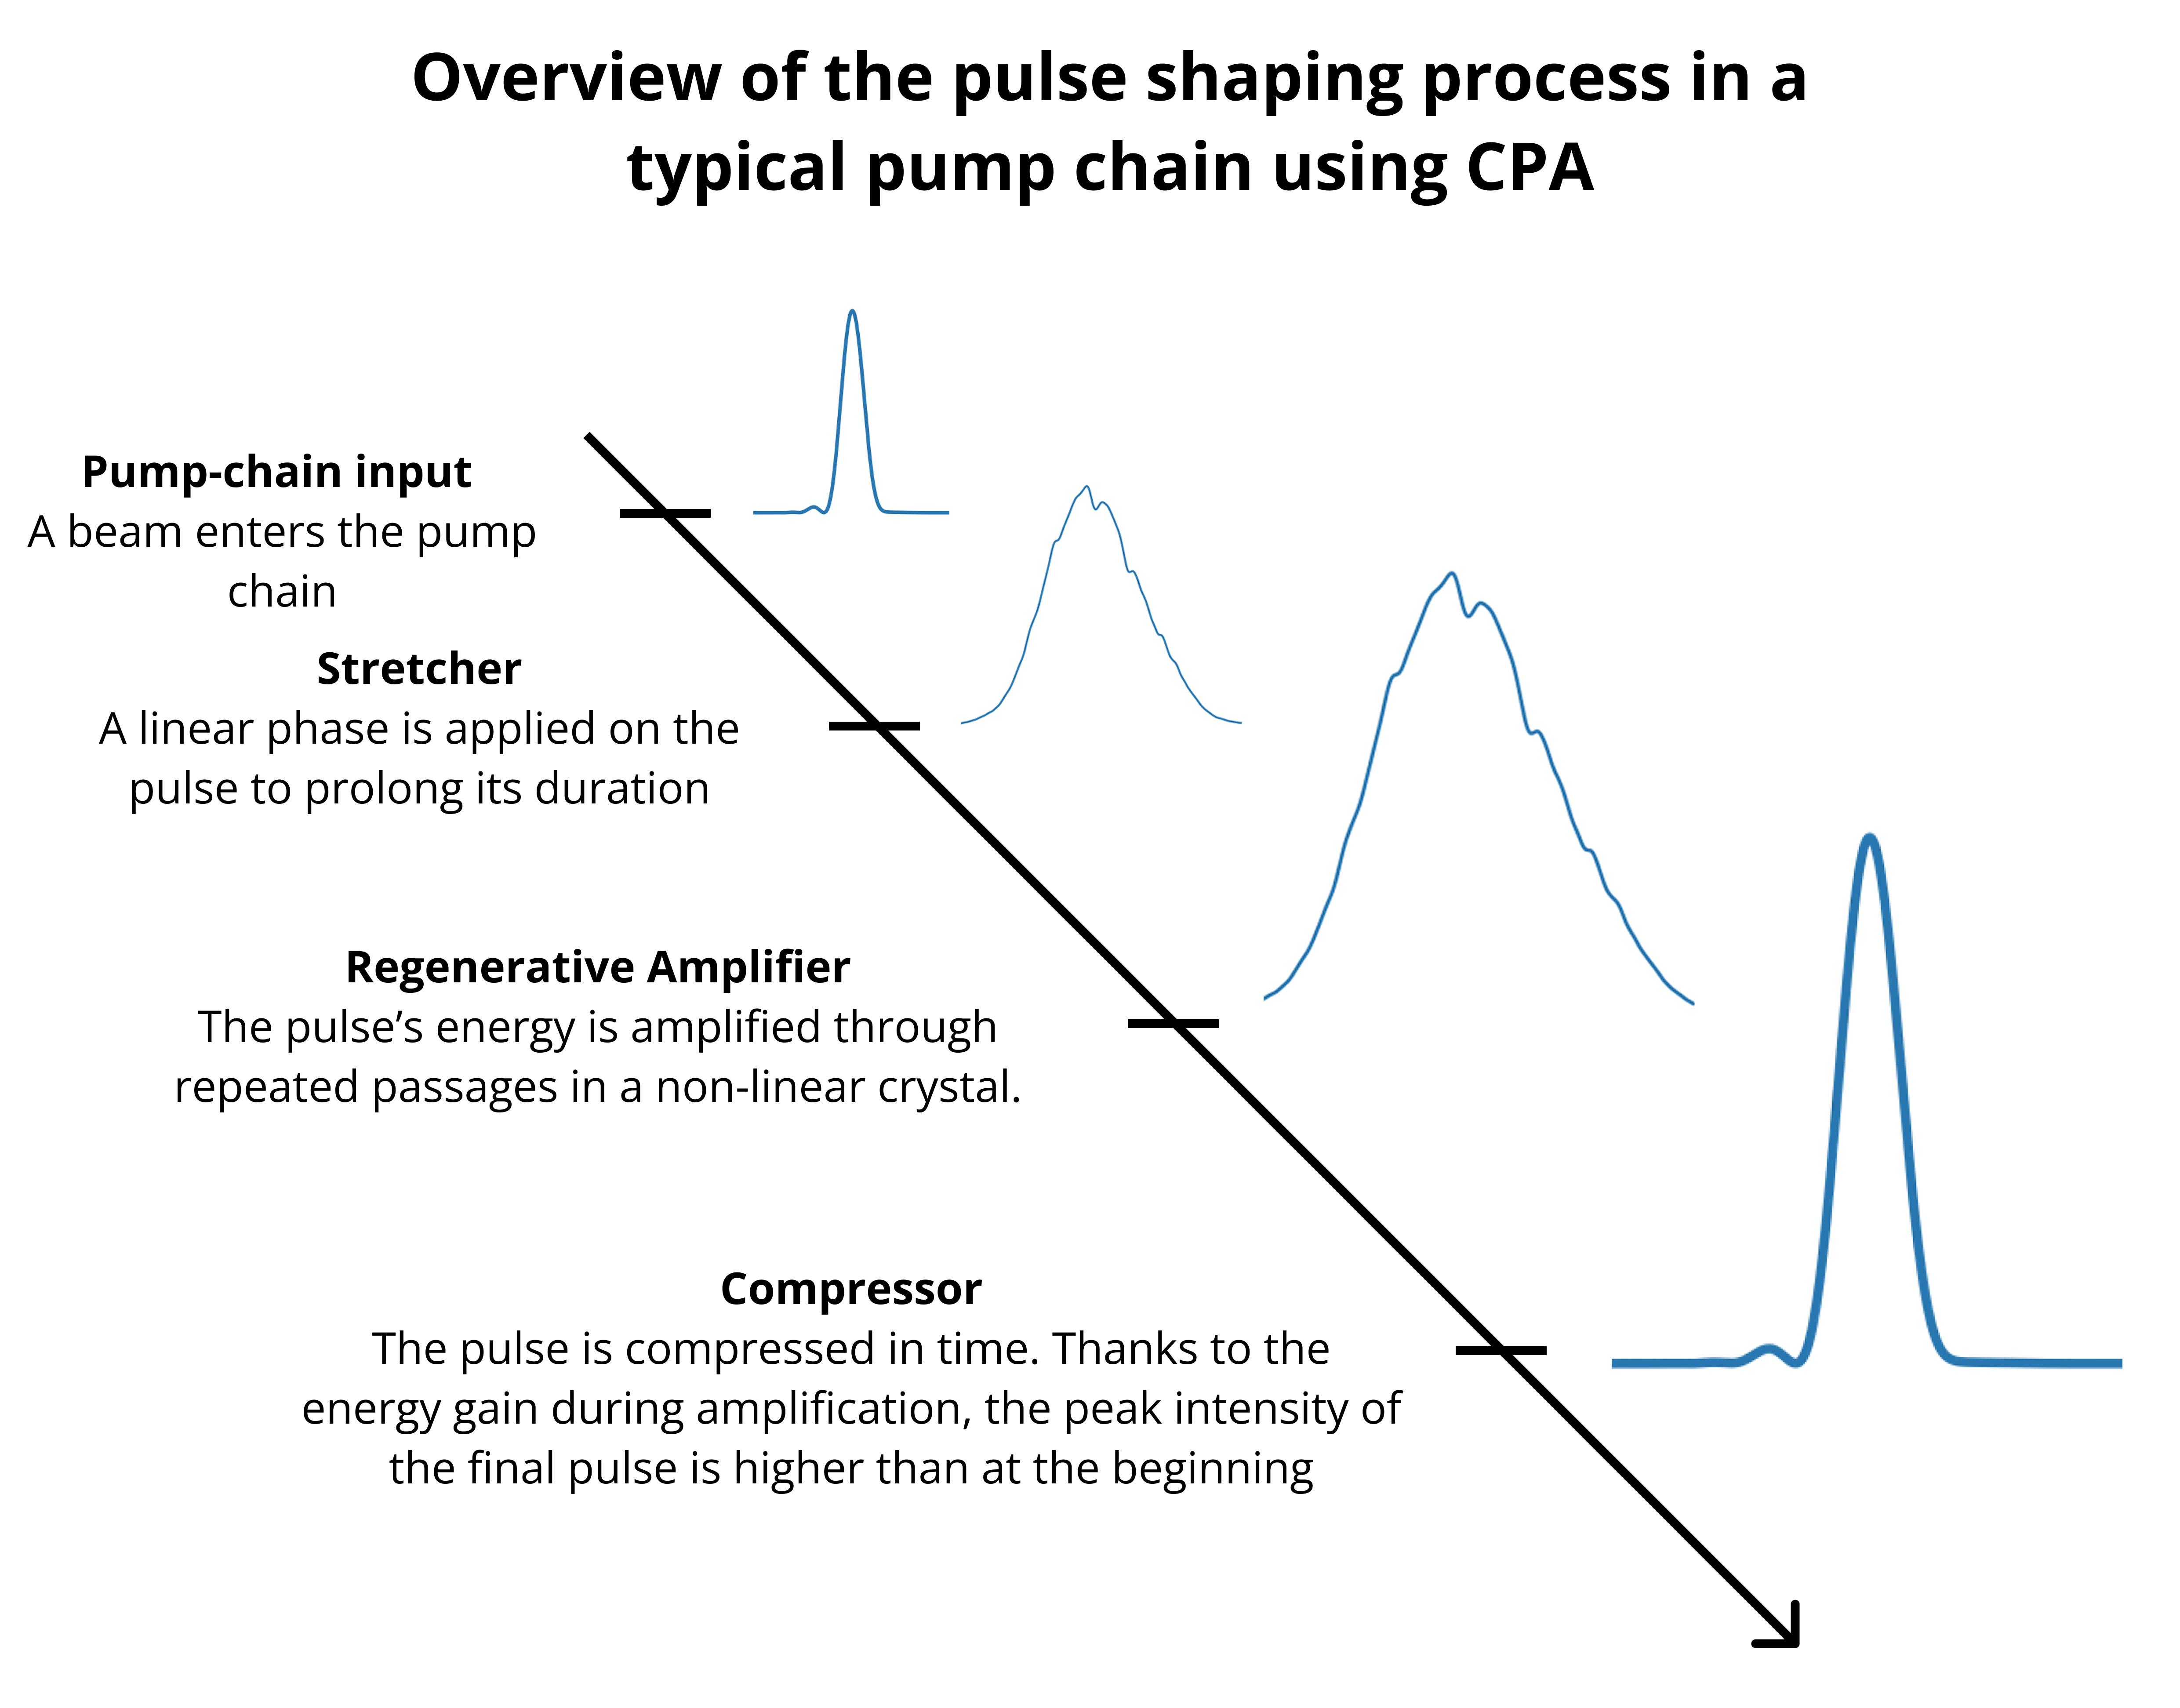
\includegraphics[width=\linewidth]{images/CPA.png}
        %     \caption{Chirped Pulse Amplification (CPA) process.}
        % \end{figure}
    \end{column}
\end{columns}
\end{frame}

%---------------------------------------
\begin{frame}{The Challenges of Pulse Shaping}
\begin{columns}[T,totalwidth=\textwidth]
    \begin{column}{0.33\textwidth}
        \centering
        \textbf{\circled{1} State Estimation} \\
        \vspace{1.25em}
        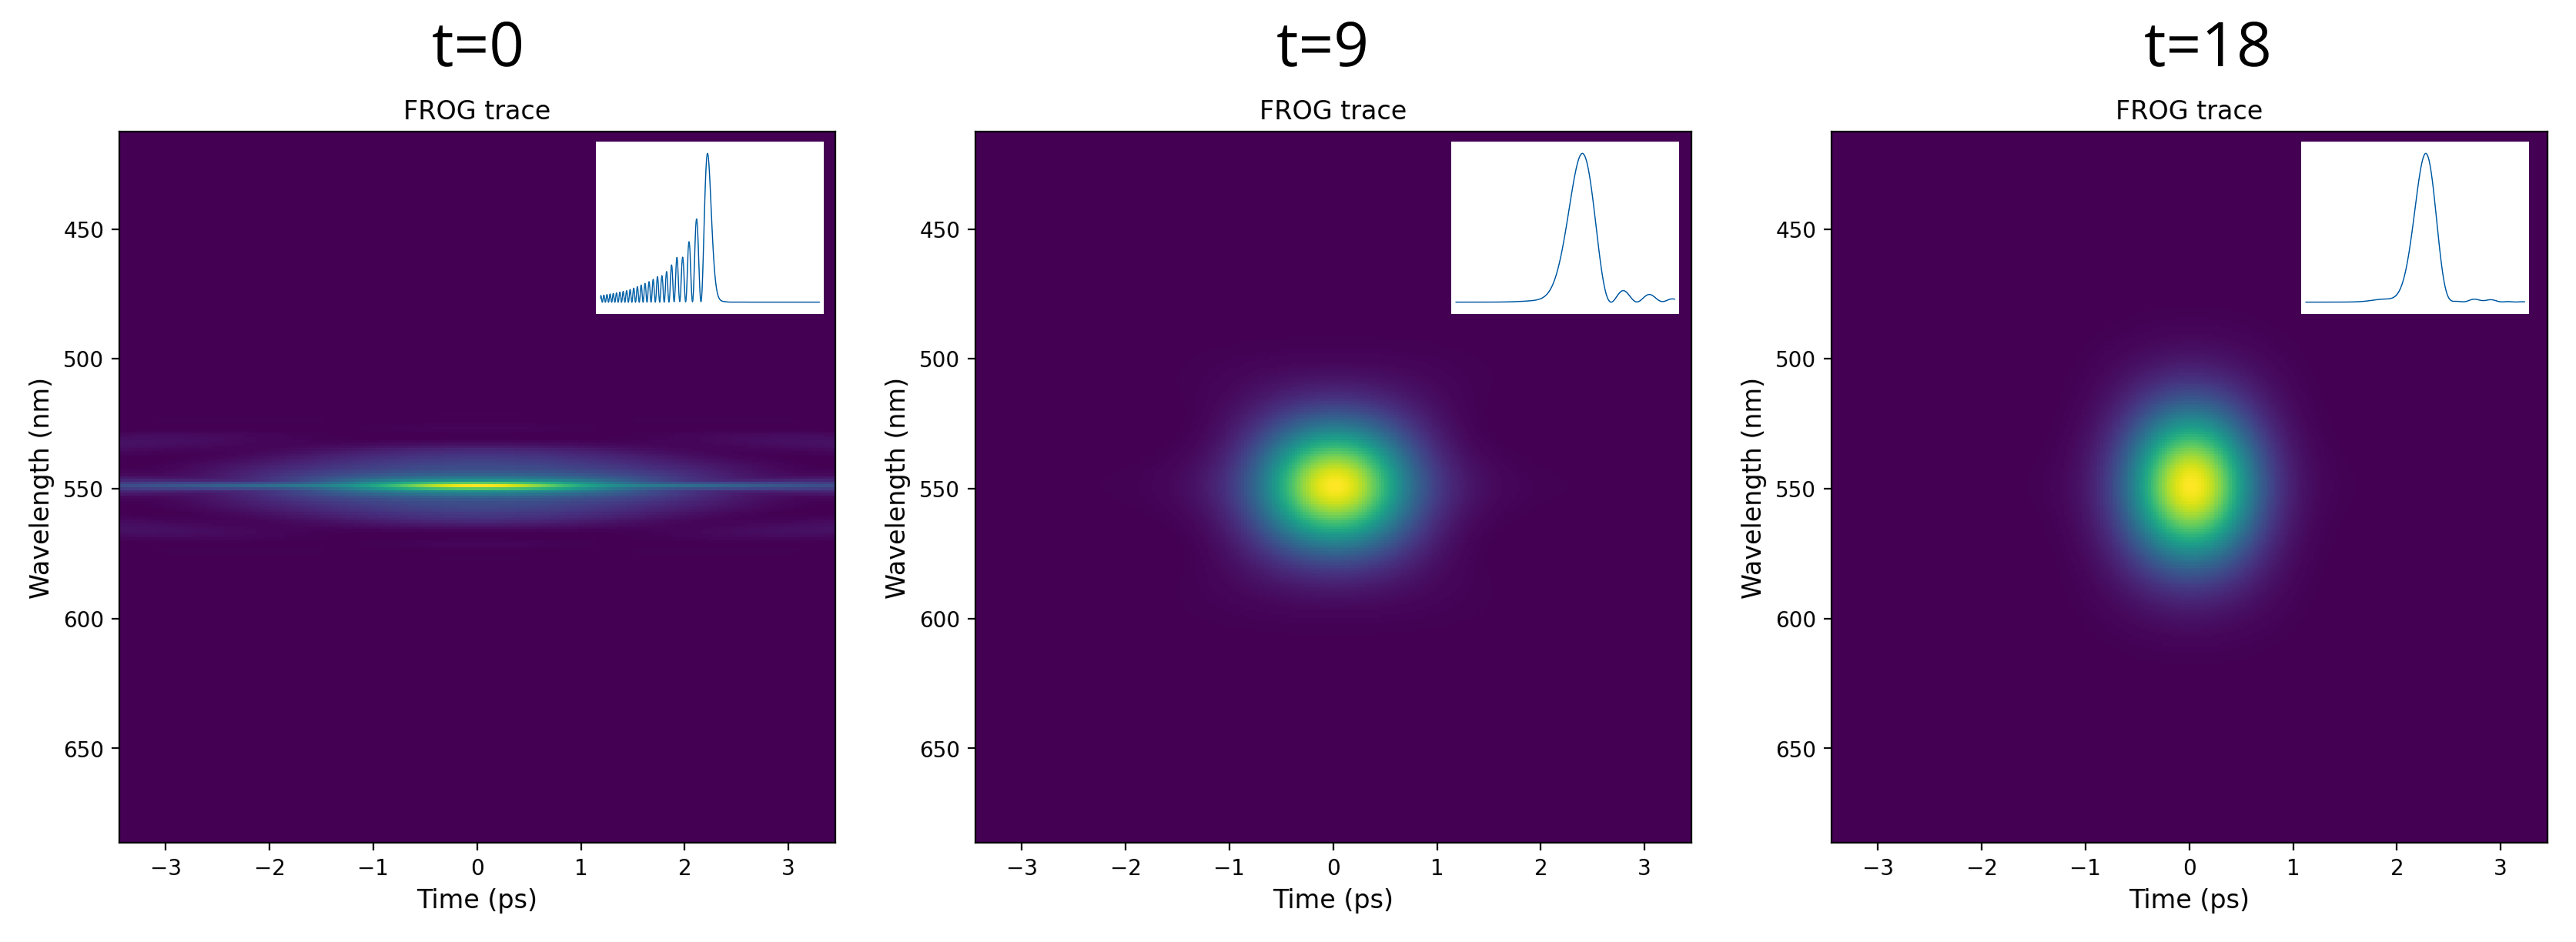
\includegraphics[width=\linewidth]{images/frogopt.png}
        \vspace{0.5em}
        Imprecise pulse reconstruction leads to poor state estimation.
    \end{column}
    \begin{column}[t]{0.33\textwidth}
        \centering
        \textbf{\circled{2} System Dynamics} \\
        \vspace{1.25em}
        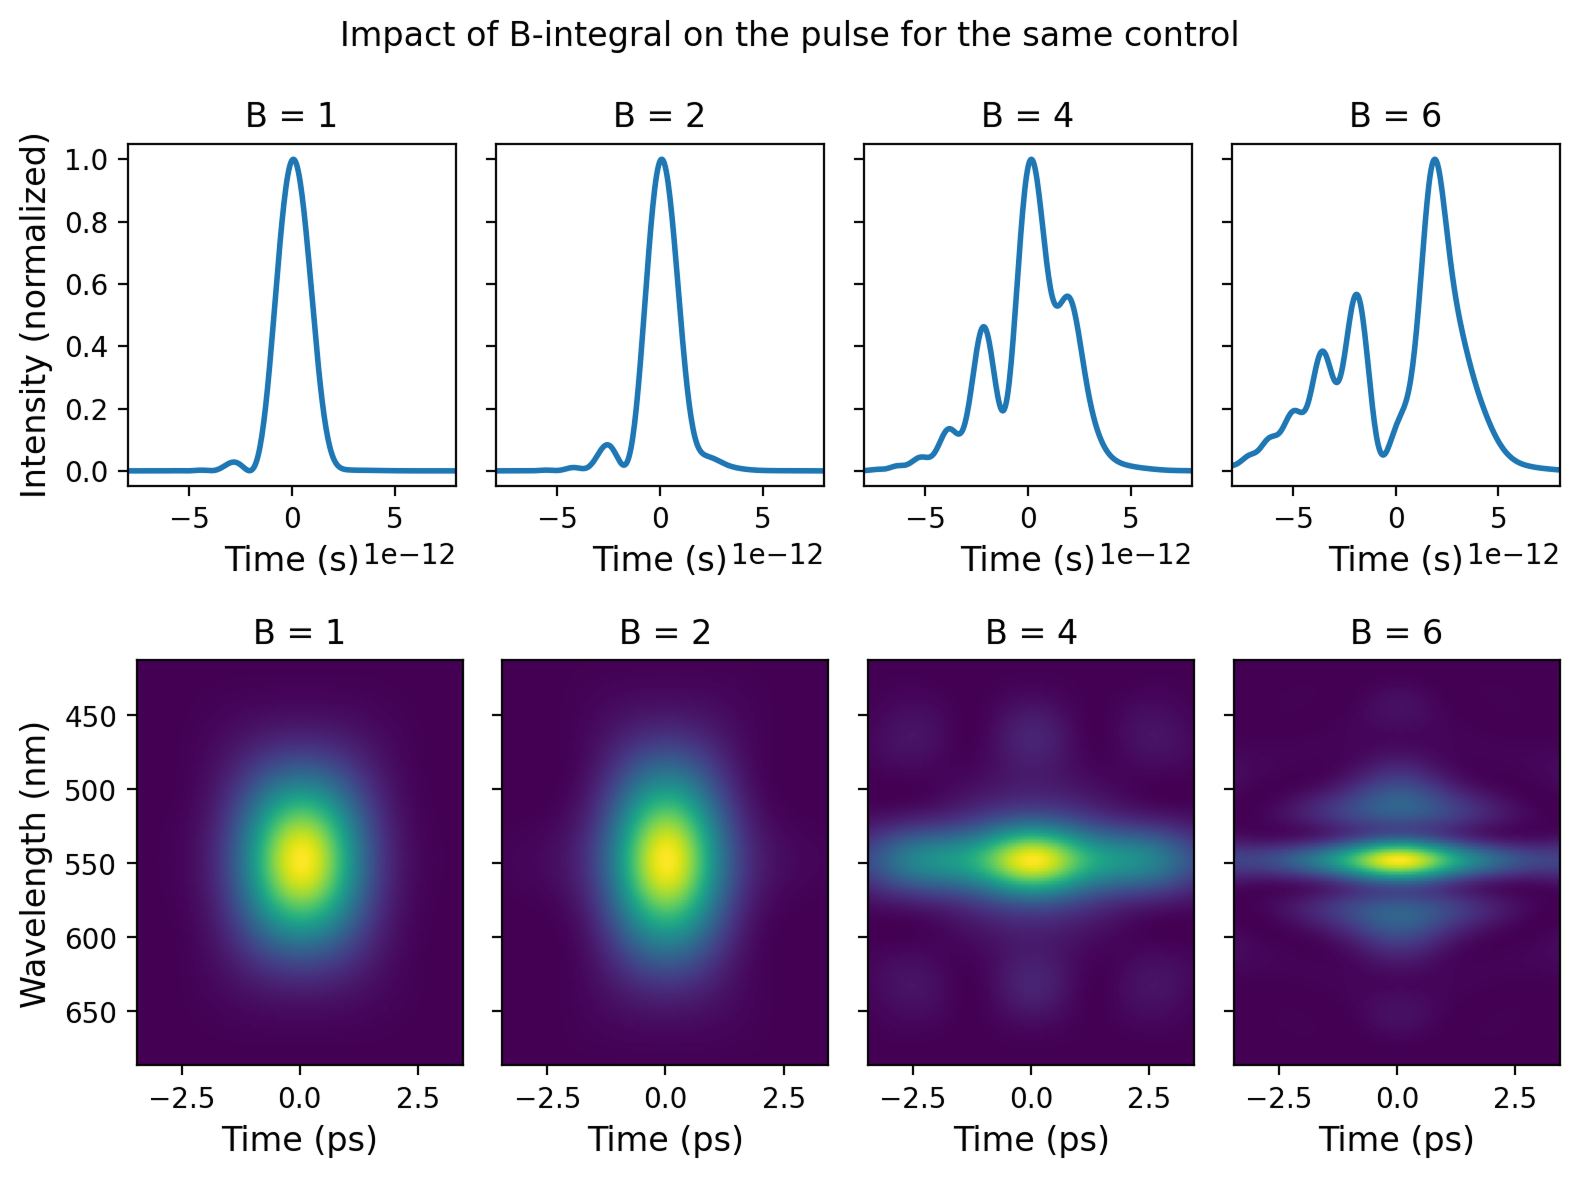
\includegraphics[width=\linewidth]{images/B_integral.png}
        \vspace{0.5em}
        Doesn't generalize well to new laser dynamics.
    \end{column}
    \begin{column}[t]{0.33\textwidth}
        \centering
        \textbf{\circled{3} Machine Safety} \\
        \vspace{1.25em}
        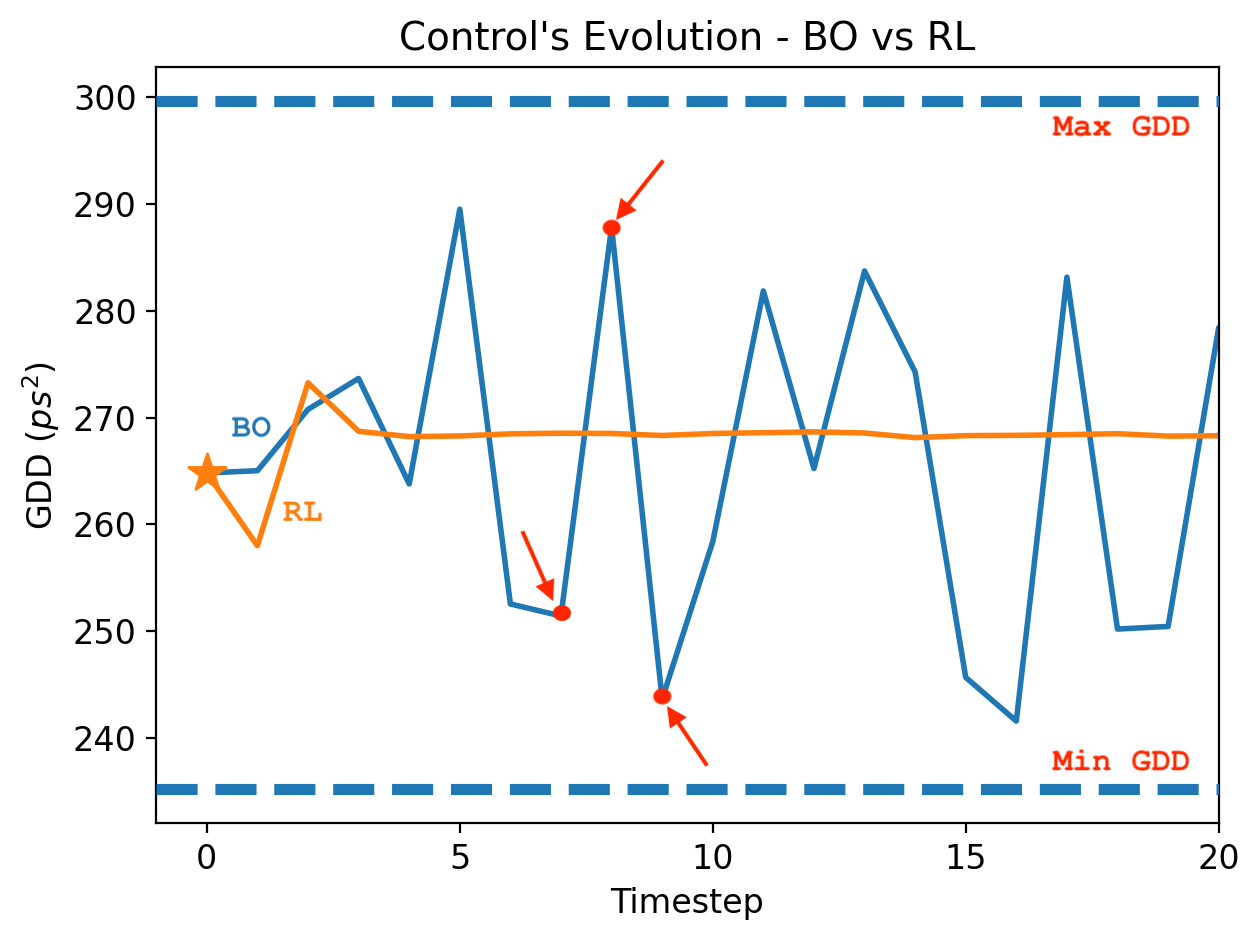
\includegraphics[width=\linewidth]{images/machinesafety.png}
        \vspace{0.5em}
        Erratic exploration can endanger the system.
    \end{column}
\end{columns}
\end{frame}
%---------------------------------------
%---------------------------------------
\begin{frame}{RL to the Rescue}
\begin{columns}[T,totalwidth=\textwidth]
    \begin{column}{0.33\textwidth}
        \centering
        \textbf{\circled{1} Learn from Images} \\
        \vspace{1.25em}
        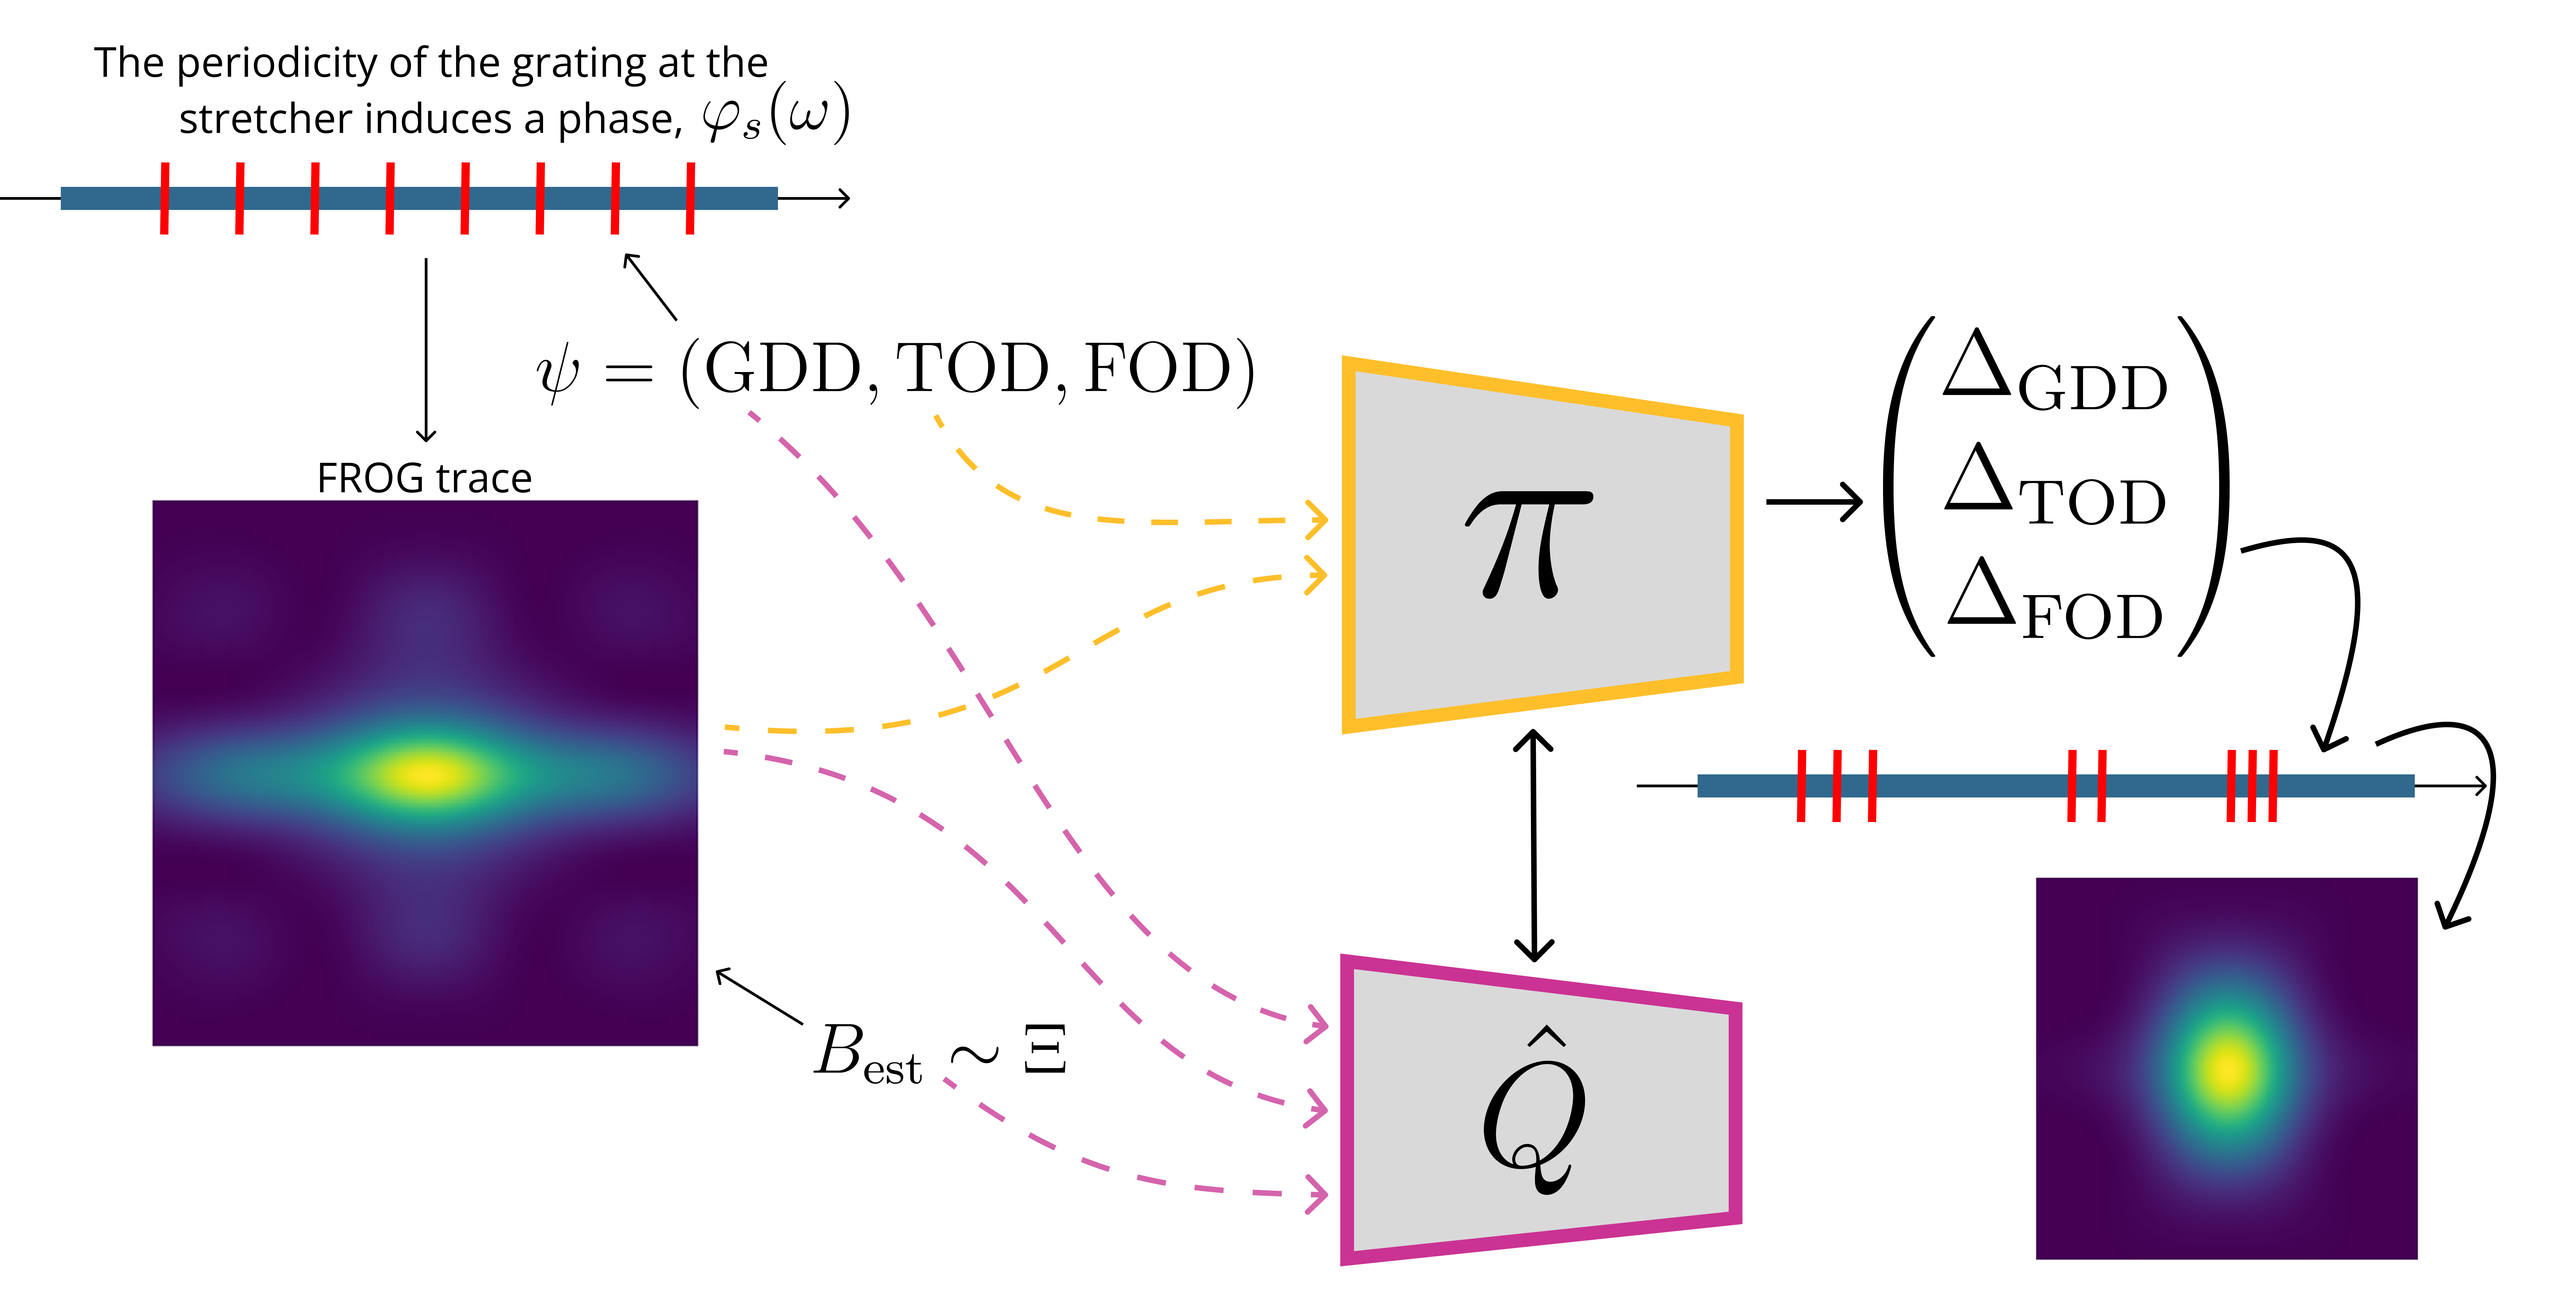
\includegraphics[width=\linewidth]{images/Figure1.png}
        \vspace{0.5em}
        Bypass noisy pulse reconstruction by learning from raw diagnostics.
    \end{column}
    \begin{column}[t]{0.33\textwidth}
        \centering
        \textbf{\circled{2} Adapt to Dynamics} \\
        \vspace{1.25em}
        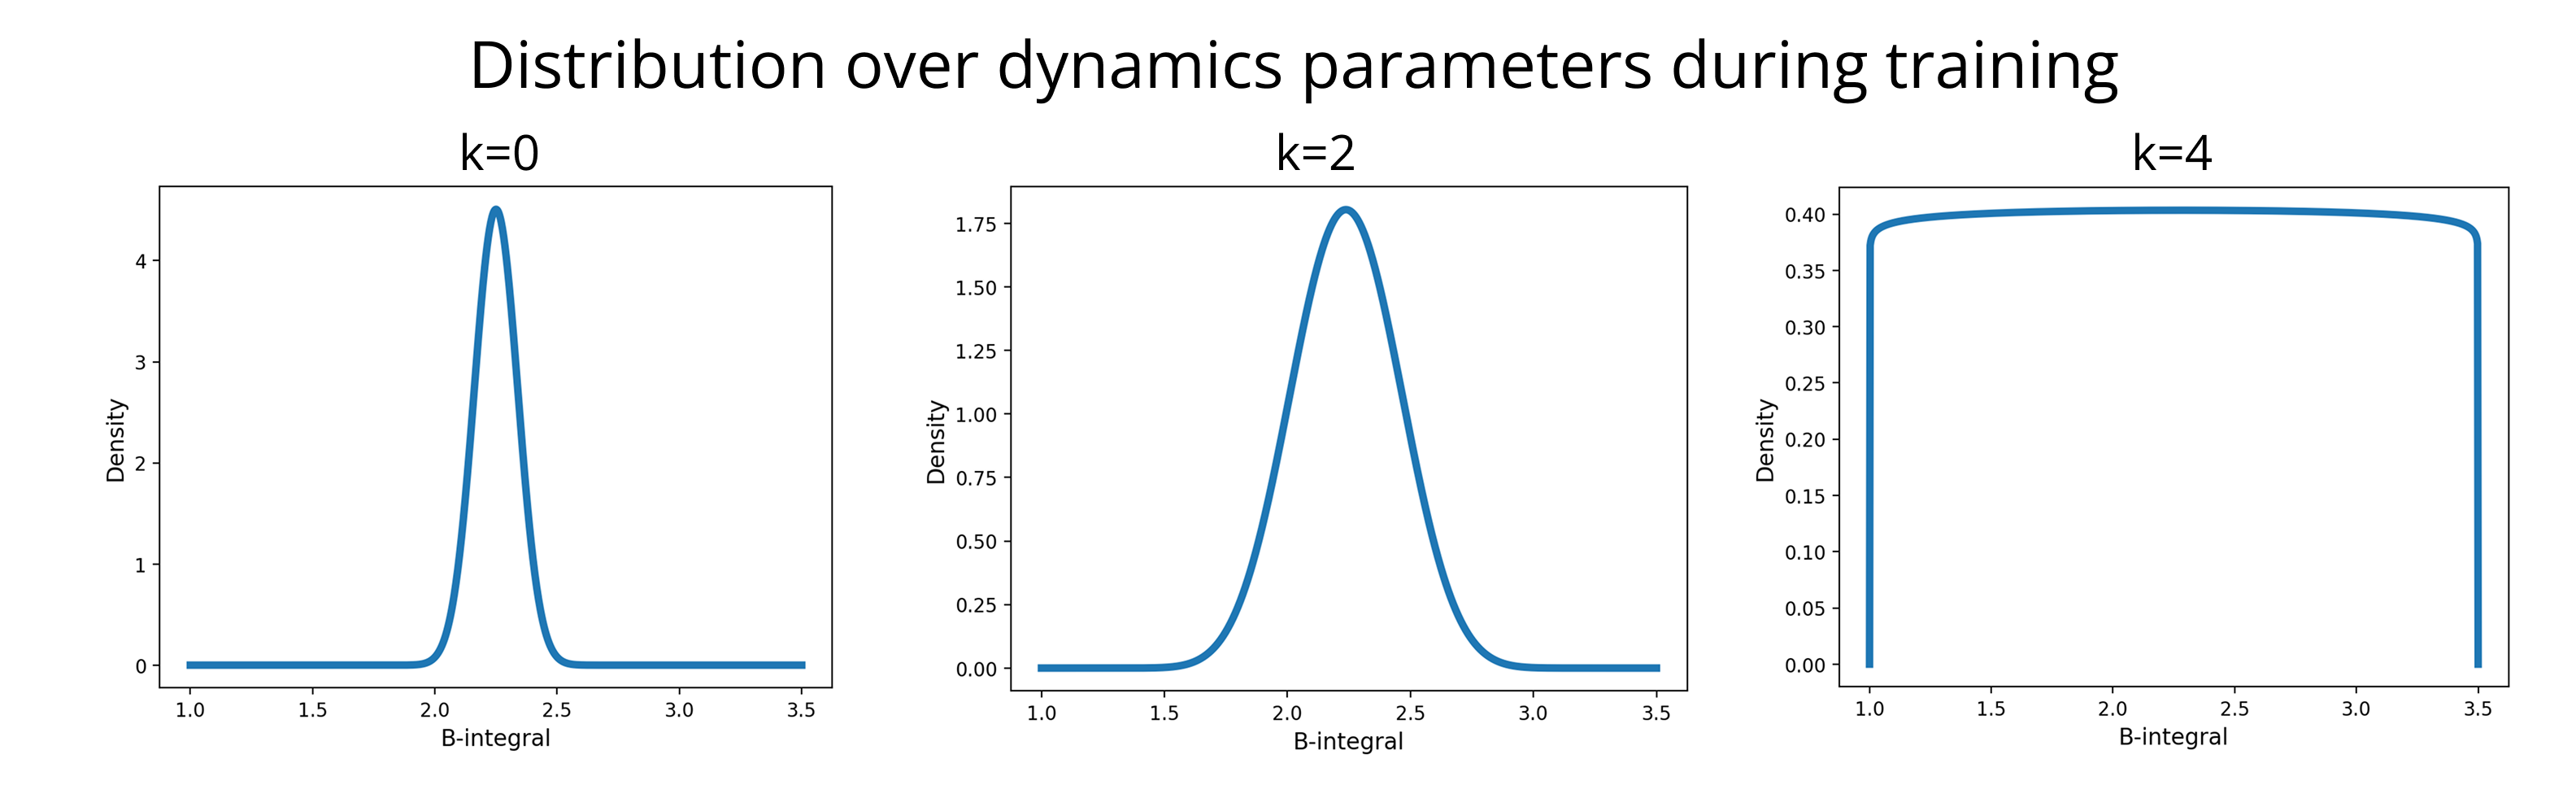
\includegraphics[width=\linewidth]{images/doraemon_distr.png}
        \vspace{0.5em}
        Train on diverse scenarios to develop robust control strategies.
    \end{column}
    \begin{column}[t]{0.33\textwidth}
        \centering
        \textbf{\circled{3} Safe Exploration} \\
        \vspace{1.25em}
        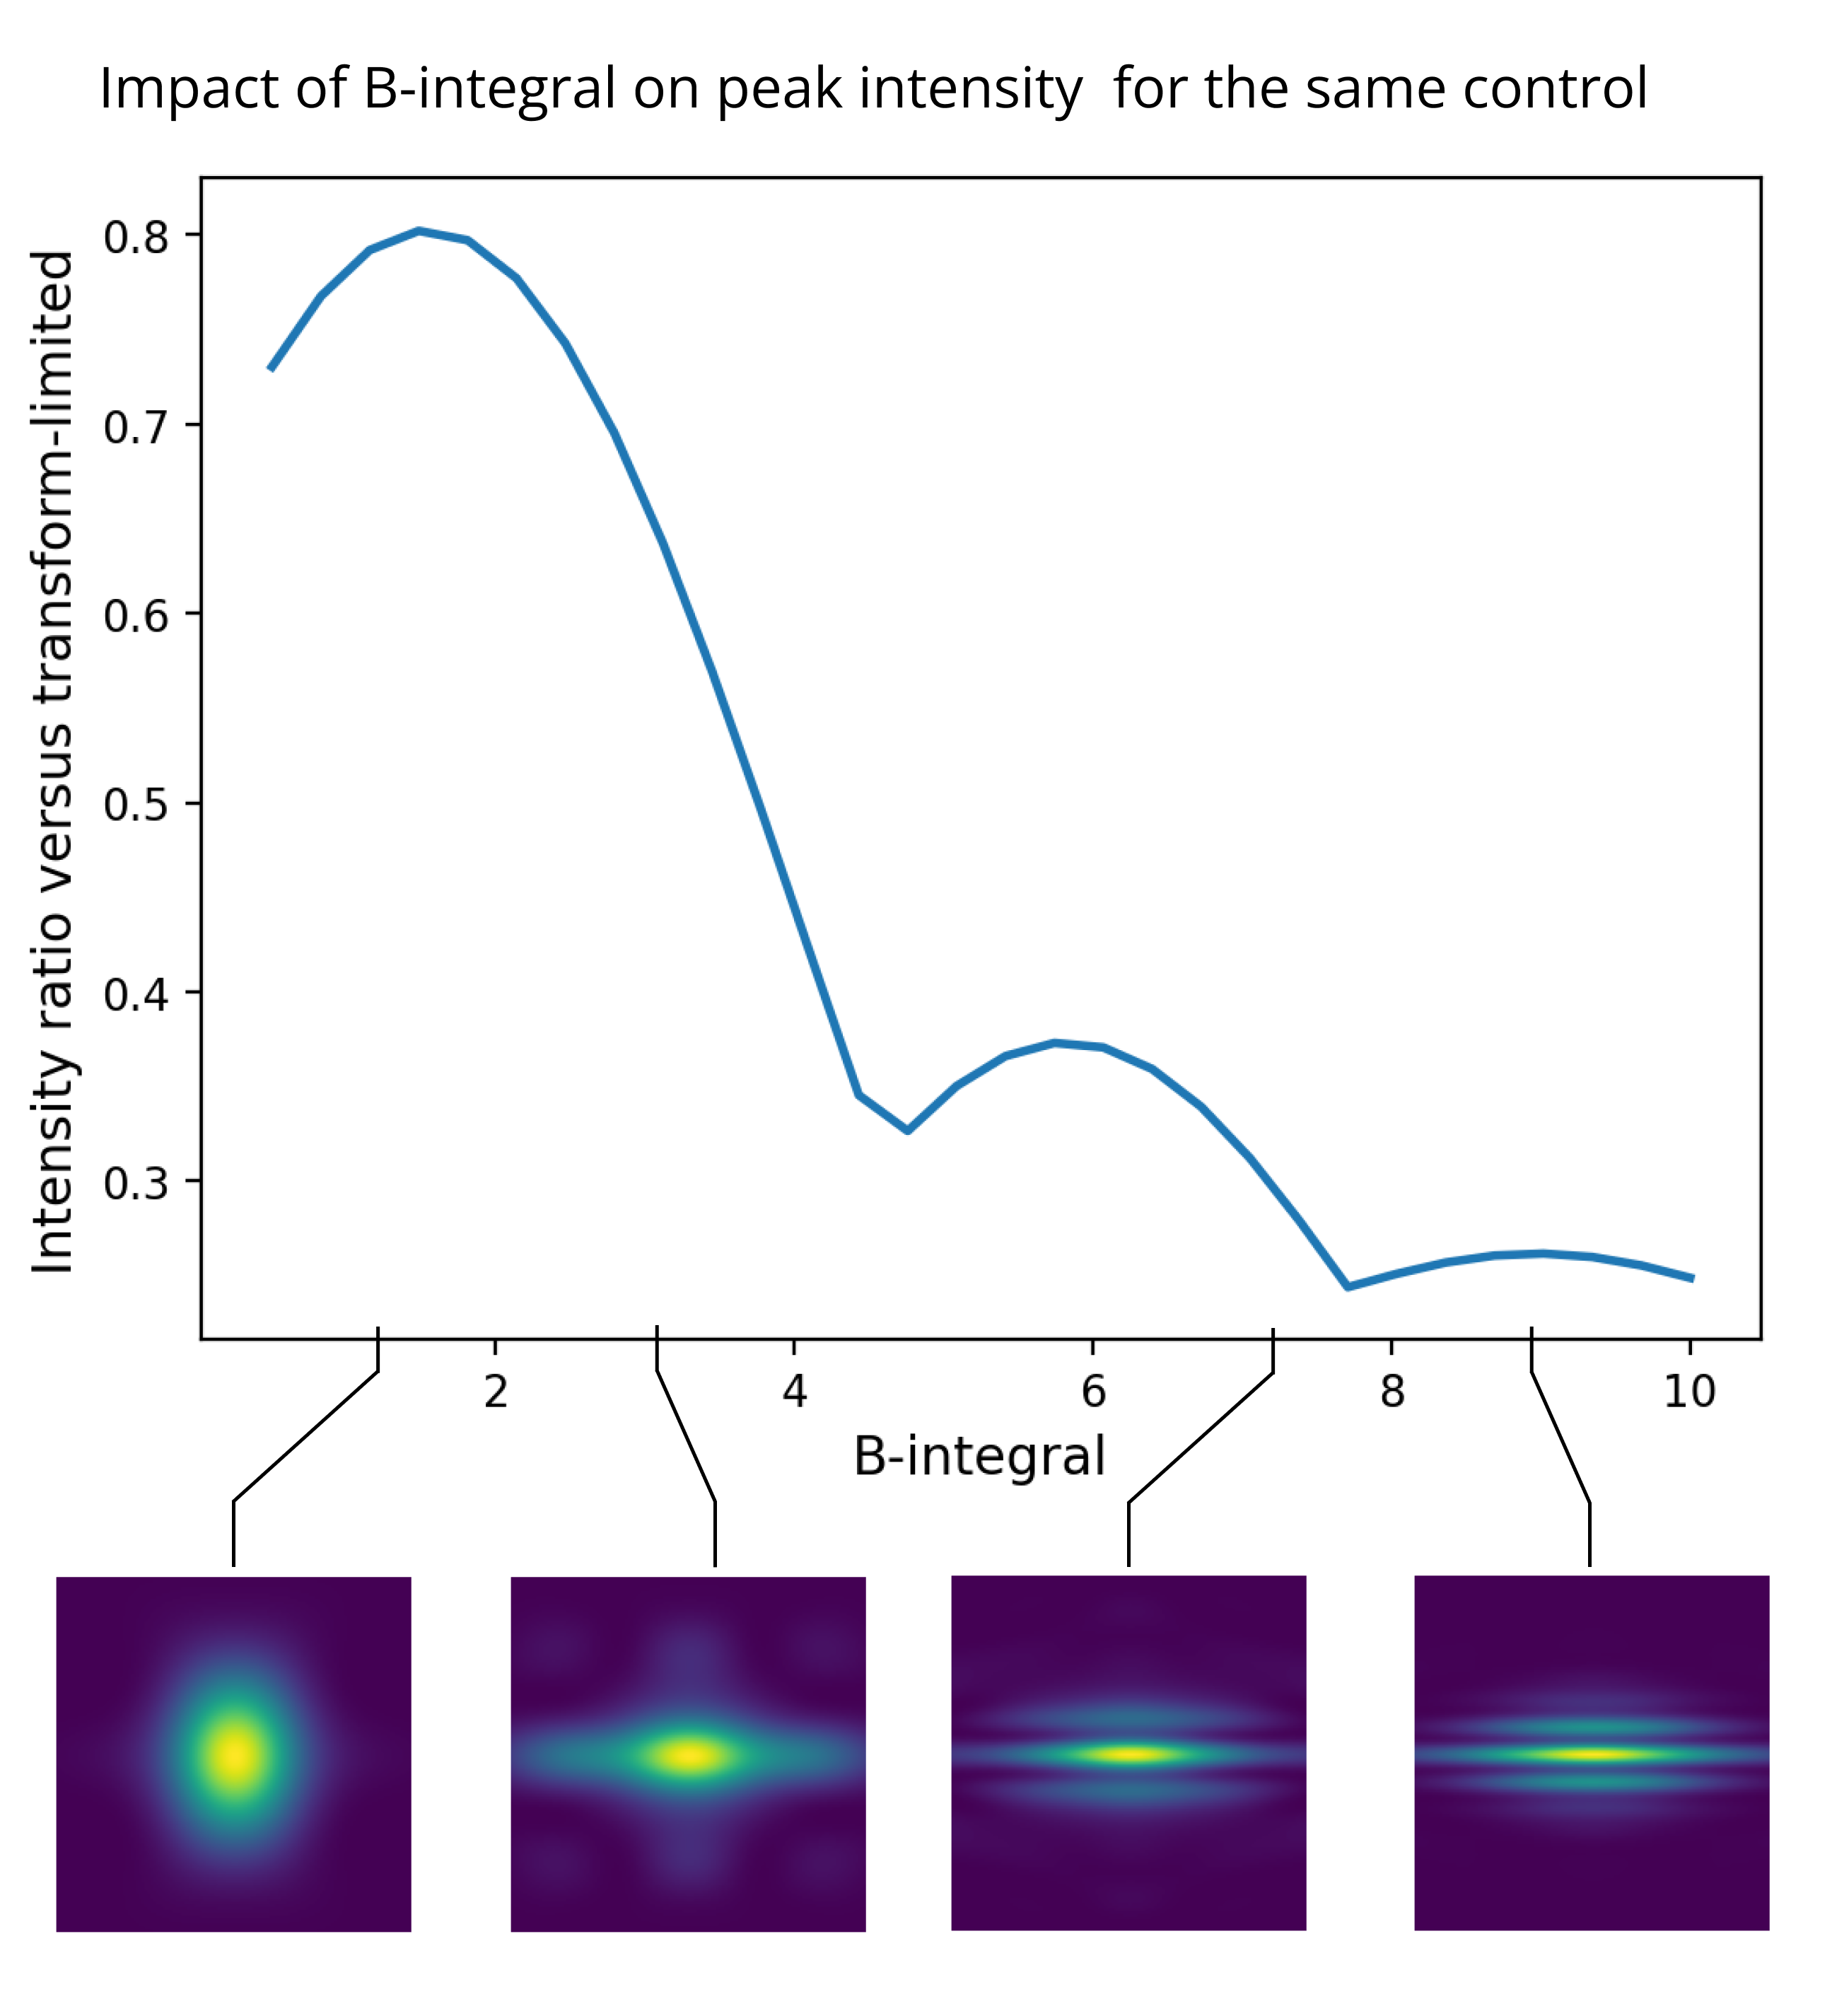
\includegraphics[width=\linewidth]{images/peak_intensity.png}
        \vspace{0.5em}
        Train in simulation to prevent erratic behavior at test time.
    \end{column}
\end{columns}
\end{frame}
%---------------------------------------
\begin{frame}{Method: Learning from Images}
\begin{columns}[T,totalwidth=\textwidth]
    \begin{column}{0.5\textwidth}
        \begin{itemize}
            \item We train an RL agent to control the laser parameters (GDD, TOD, FOD).
            \item The agent receives a FROG trace image as input.
            \item It outputs a change in the laser parameters.
            \item The goal is to maximize the peak intensity of the laser pulse.
        \end{itemize}
    \end{column}
    \begin{column}{0.5\textwidth}
        % \begin{figure}
        %     \includegraphics[width=\linewidth]{images/Figure1_and_CPA_edit.png}
        %     \caption{The RL agent learns to map FROG images to laser parameter adjustments.}
        % \end{figure}
    \end{column}
\end{columns}
\end{frame}
%---------------------------------------
\begin{frame}{Experimental Results}
\begin{columns}[T,totalwidth=\textwidth]
    \begin{column}{0.5\textwidth}
        \centering
        \textbf{Adapting to Dynamics}
        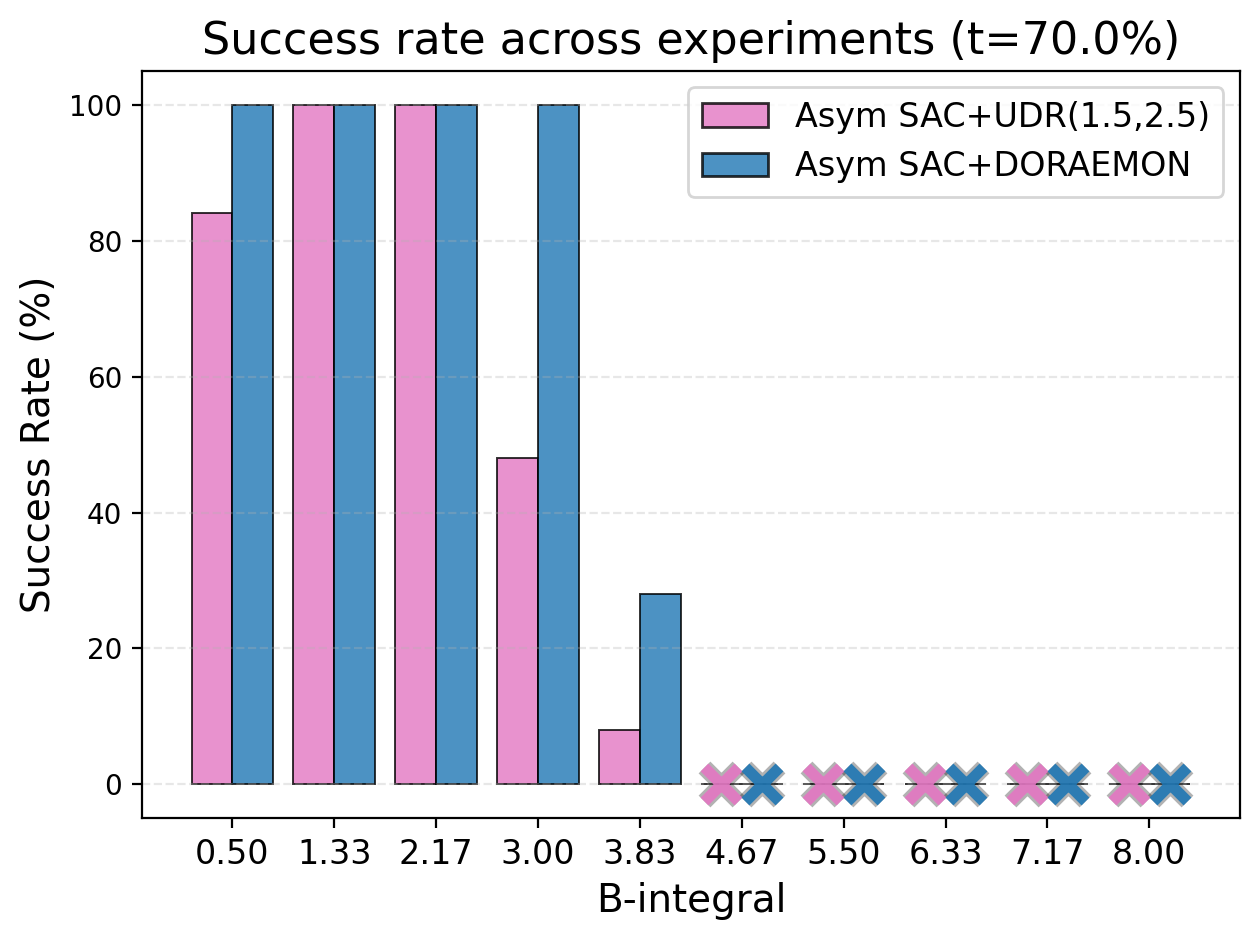
\includegraphics[width=\linewidth]{images/doraemon_vs_udr_succ_rate_70.png}
        Our method (DORAEMON) maintains high performance.
    \end{column}
    \begin{column}{0.5\textwidth}
        \centering
        \textbf{Peak Intensity}
        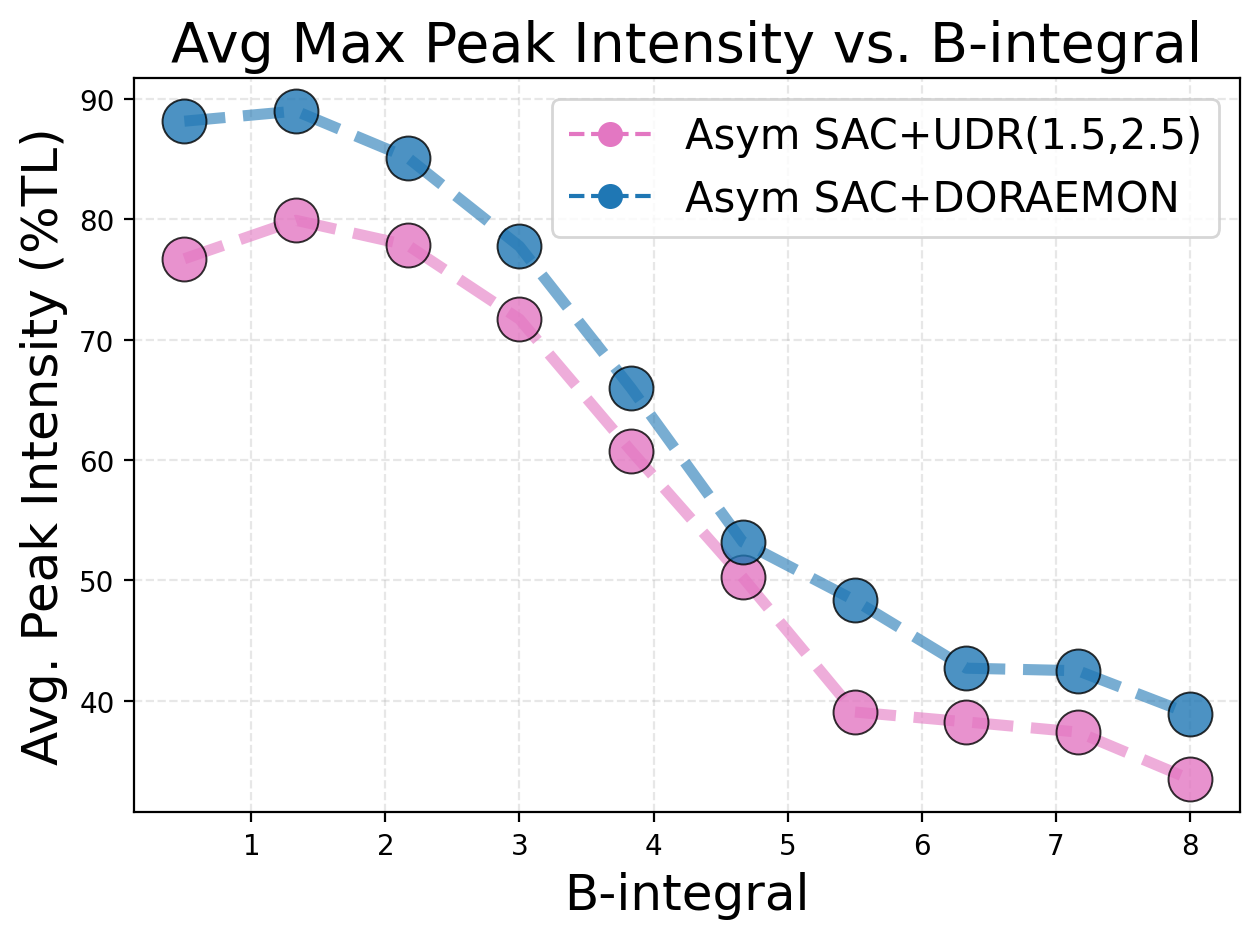
\includegraphics[width=\linewidth]{images/udr_vs_doraemon_average.png}
        Our method achieves higher peak intensity.
    \end{column}
\end{columns}
\end{frame}
%---------------------------------------
\begin{frame}{Conclusions}
\begin{itemize}
    \item We present a new method for shaping laser pulses using RL.
    \item Our method learns from images, bypassing noisy reconstruction.
    \item It is robust to changes in the laser's dynamics.
    \item It is trained in simulation, ensuring safe exploration.
    \item Our results show that our method outperforms existing baselines.
\end{itemize}
\end{frame}
% ----------------------------------------
\begin{frame}[allowframebreaks]{References}
  \small
  \bibliographystyle{plainnat}
  \bibliography{main} 
\end{frame}
% ----------------------------------------
\end{document}
